\documentclass[11pt,a4paper,english]{uvamath}
\usepackage[english]{babel}

\usepackage{amsmath, amsfonts, amssymb, a4wide, fancyhdr, lineno, graphicx, epsfig, soul, color, hyperref}
\usepackage[square, numbers]{natbib}

% Running line numbers:
\linenumbers
% Number only every 5:th line:
\modulolinenumbers[5]

%Nodig om een bibliography midden in het artikel te zetten, ipv aan het einde zoals eigenlijk gebruikelijk is
\renewcommand{\bibsection}{}

% TODO command
\newcommand{\todo}[1]{
    \hl{#1}
}

% The things that should be filled in by each group, depending on their situation, are written in a todo command, \todo{like this text}. All text in normal the normal font, is applicable for any group. However, everyone is free to adapt any text, and it is even suggested to look at all text critically and make changes if needed.

% Project specific commands
\author{Tom van Duist \& Kevin van den Bekerom}

\newcommand{\projectname}{\todo{Project Name}\ }


\newcommand{\aanpassen}[1]{ {\sethlcolor{green} \hl{#1}} }

\title{Reading assignment week 3}
%Variables
\newcommand{\TitelAbbr}{}
\newcommand{\Version}{0.1}



\what{}
\supervisors{}
\author{Tom van Duist}


\begin{document}

\maketitle
\clearpage


\chapter*{Reading assignment week 3}

\section*{4.1}

\subsection*{Transformational \cite{req_en_book}}
Based on the requirements a formal specification is defined. This is progressively developed until a working system can be derived from the formal definition. The system (or part of it) is generated automatically from the formal specifications.
\begin{itemize}
	\item[\textbf{+}] System automatically generated from formal specifications.
	\item[\textbf{+}] Theoretically, if the specification is verified, the resulting system has no defects.
	\item[\textbf{+}] Specification and implementation will not diverge.
	\item[\textbf{-}] Difficult to manipulate the (formal) specifications.
	\item[\textbf{-}] Only applicable to very specific systems.
	\item[\textbf{-}] Need sophisticated development tools.
\end{itemize}
\begin{figure}[h]
	\centering
	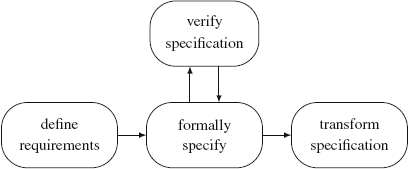
\includegraphics[width=0.75\linewidth]{Resources/4_transformational.png}
	\caption{The transformational process model.}
	\label{fig:transformational}
\end{figure} 

\clearpage
\subsection*{Spiral \cite{req_en_book}}
Based on a risk-driven approach instead of documents or code and centres on the identification and elimination of problems with high risk. Tasks are organised in cycles, where each cycle constitutes of four tasks.
\begin{itemize}
	\item[\textbf{+}] Could remove some of the risks associated with big projects.
	\item[\textbf{+}] When the requirements (after n cycles) are known a different process can follow.
	\item[\textbf{-}] Adds significant effort to the definition and development process.
	\item[\textbf{-}] Meta-model used to instantiate different process models.
\end{itemize}
\begin{figure}[h]
	\centering
	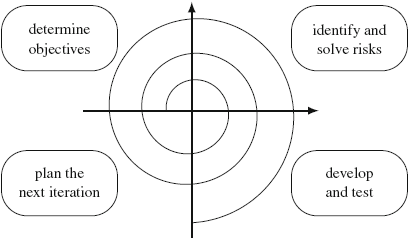
\includegraphics[width=0.75\linewidth]{Resources/4_spiral.png}
	\caption{The spirals model.}
	\label{fig:transformational}
\end{figure} 


\chapter{References}

\begin{thebibliography}{9}
	
	\bibitem{req_en_book}
	Joao M. Fernandes, Ricardo J. Machado, \\
	\emph{Requirements in Engineering Projects}
	
\end{thebibliography}


\appendix


\end{document}
